\section{Valutazione} \label{sec:val}
Al termine dello sviluppo di \acs{gea} siamo riusciti ad ottenere un incontro presso il centro terapeutico in modo da poter testare il gioco sul campo e ricevere feedback e suggerimenti da parte di terapeuti e ragazzi.\\
Il giorno 19 Gennaio 2018 in una stanza del centro terapeutico "Fraternità e amicizia" abbiamo effettuato tre sessioni di test: la prima è stata svolta facendo provare il gioco agli specialisti del centro mentre le successive due coinvolgevano gruppi da 6/7 ragazzi ciascuno. Grazie all'utilizzo di Google Chromecast abbiamo potuto replicare lo schermo dello smartphone su un televisore così che anche chi non stava giocando poteva vedere come funzionavano i singoli mini-giochi. Tutti i ragazzi sono stati entusiasti e hanno voluto sperimentare tutti i giochi, nessuno di loro ha avuto sensazioni di nausea o fastidi causati da questo primo approccio alla realtà virtuale. \acs{gea} ha dunque suscitato grande interesse e ammirazione da parte di tutti gli utenti i quali hanno espressamente detto di volerlo continuare ad usare nelle loro sedute. I tempi di apprendimento del funzionamento e di gioco sono risultati similari in tutti coloro che hanno sperimentato per cui si può affermare che sia di facile utilizzo e comprensione ad eccezione del mini-gioco "E' sano o no?" in quanto risulta più difficile capire come trascinare l'elemento da buttare nella spazzatura. Per quanto riguarda i punteggi ottenuti anch'essi si sono rivelati nella norma e spesso molto elevati. Abbiamo inoltre notato che anche i ragazzi che non stavano sperimentando in prima persona venivano coinvolti grazie alla visione del gioco sullo schermo del televisore ed incitavano il compagno nelle scelte da prendere. \acs{gea}, pensato inizialmente come gioco individuale, è risultato invece molto efficace anche come gioco di gruppo e di squadra basato sull'aiuto reciproco e la collaborazione. \\
Di seguito vi sono delle foto scattate durante la mattinata sopracitata e gentilmente concesse dal centro "Fraternità e amicizia".
\begin{figure*}
 \begin{minipage}[c]{\columnwidth}
   \centering
   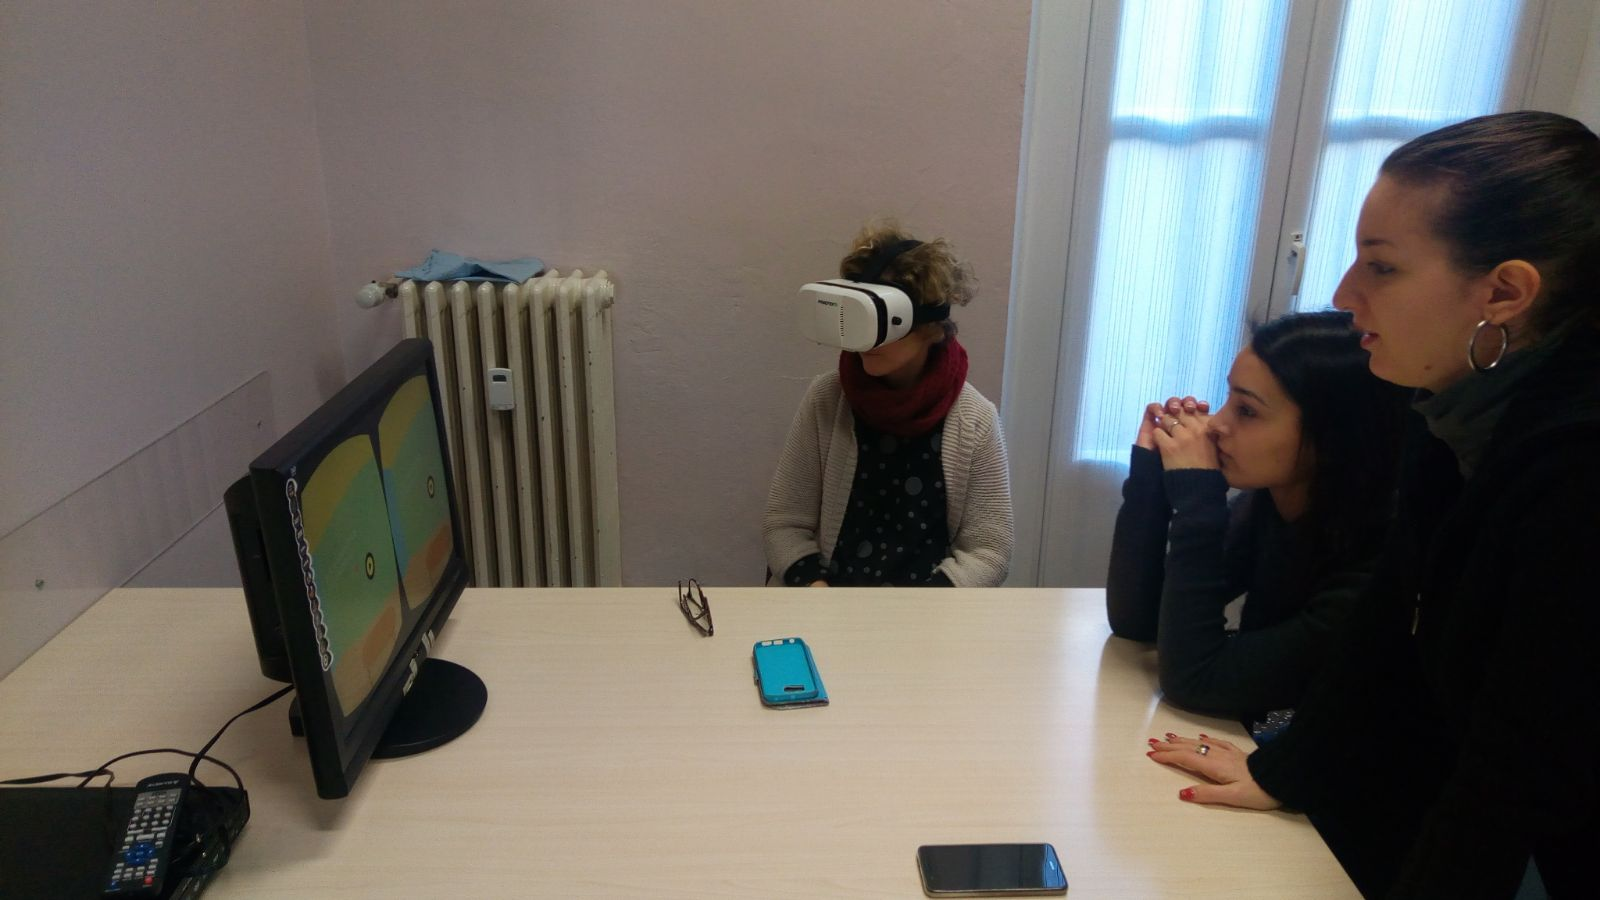
\includegraphics[width=8cm]{Images/terap}
   \caption{Prima sessione di test: Una terapeuta prova il gioco alla nostra presenza}
   \label{fig:test1}
 \end{minipage}
 \ \hspace{8mm} \hspace{8mm} \\\
 
 \begin{minipage}[c]{\columnwidth}
  \centering
   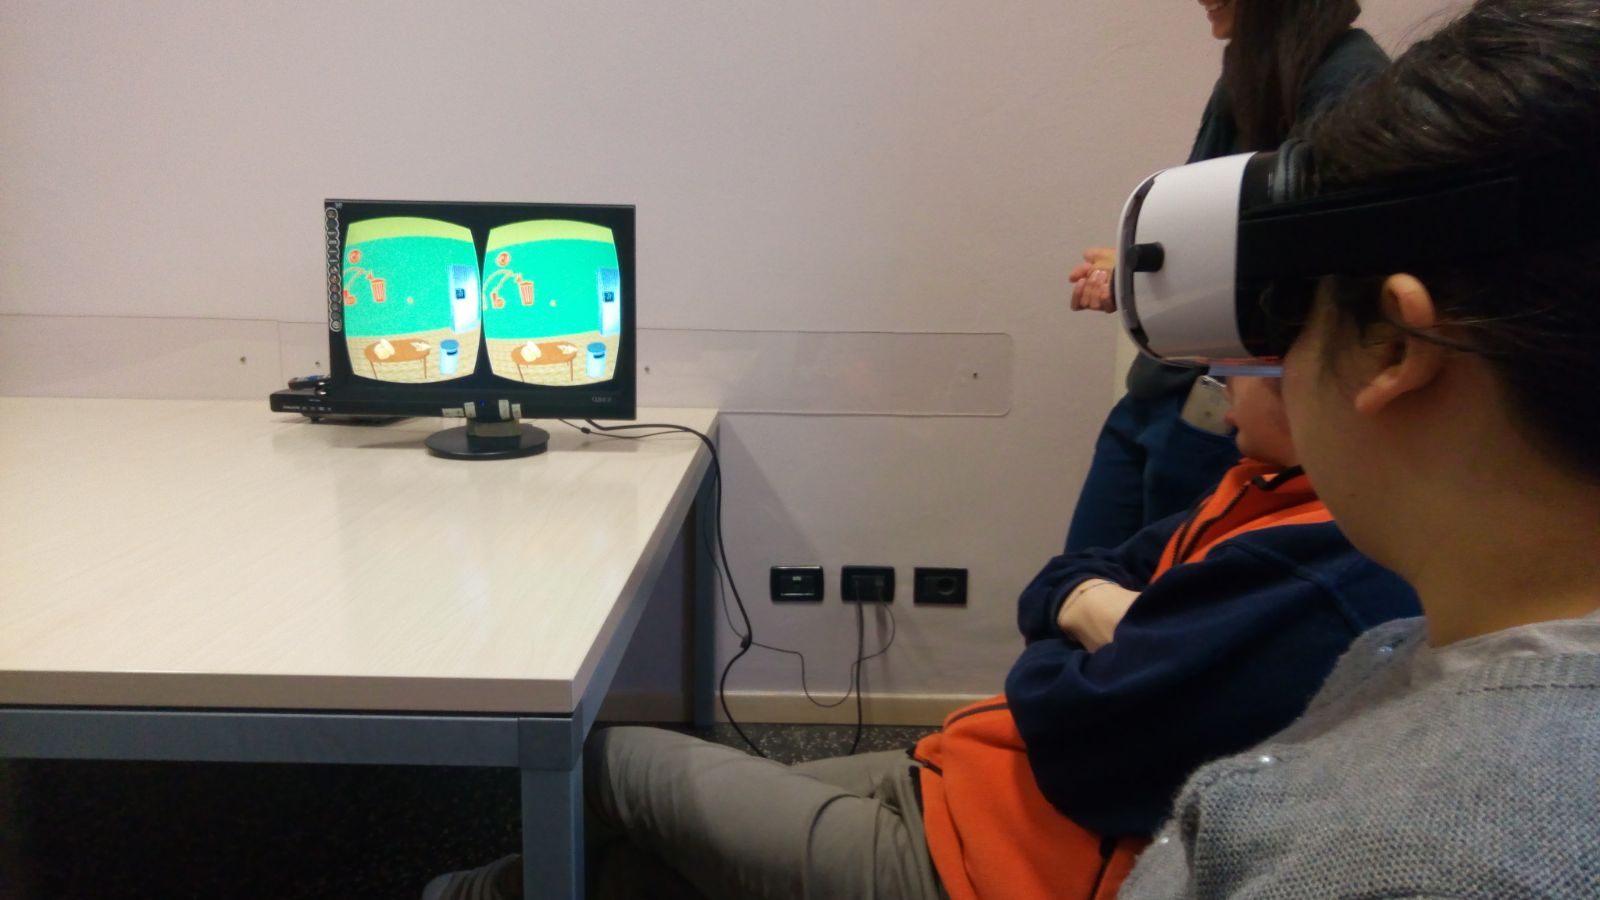
\includegraphics[width=8cm]{Images/raga}
   \caption{Seconda sessione di test: Una ragazza prova il gioco mentre gli altri osservano il televisore}
   \label{fig:test2}
 \end{minipage}
 \ \hspace{8mm} \hspace{8mm} \\\
 
 \begin{minipage}[c]{\columnwidth}
  \centering
   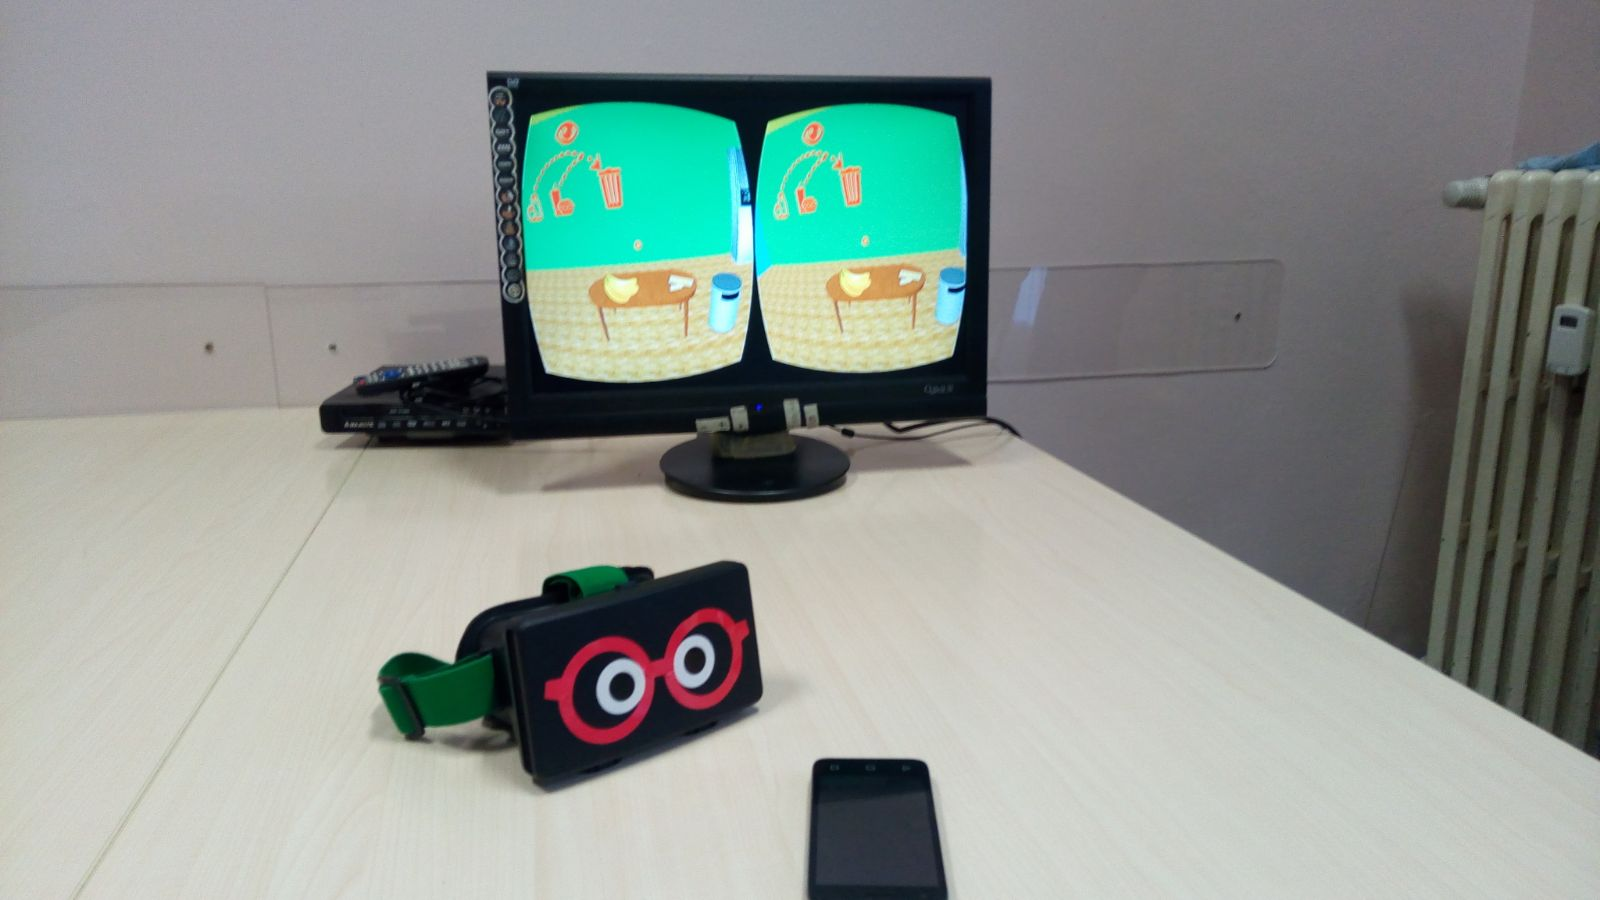
\includegraphics[width=8cm]{Images/strumenti}
   \caption{Primo piano dello schermo del televisore}
   \label{fig:tele}
 \end{minipage}
\end{figure*}
\clearpage

La nostra soluzione risulta essere una buona soluzione per svariate motivazioni quali:
\begin{itemize}
\item[->] La realtà virtuale permette di avere un ampio database con la presenza di tutti i possibili alimenti senza dover usare vero cibo che andrebbe quindi poi sprecato;
\item[->] \acs{gea} risulta essere una soluzione compatta in quanto si necessita solamente di uno smartphone, al giorno d'oggi posseduto dalla maggior parte della popolazione, e un visore \acs{vr}, acquistabile con una spesa minima, per cui facilmente trasportabile;
\item[->] \acs{gea}, per via della facile reperibilità della tecnologia utilizzata, permette al bambino di poter continuare la sua educazione in campo alimentare anche in completa autonomia a casa propria senza dover aspettare di andare al centro nella giornata dedicata al laboratorio di alimentazione;
\item[->] Grazie alla presenza di una grafica simpatica e colorata questa applicazione permette di avere un'esperienza divertente motivando i bambini nell'imparare giocando;
\item[->] Grazie all'uso di Google Chromecast è possibile avere due sedute in una: una seduta individuale svolta dal ragazzo che indossa il visore e gioca e una seduta di gruppo per i ragazzi seduti attorno che osservano lo schermo del televisore. Permette quindi training individuale e di gruppo nello stesso momento.
\end{itemize}